\documentclass{amia}
\usepackage{graphicx}
\usepackage[labelfont=bf]{caption}
\usepackage[superscript,nomove]{cite}
\usepackage{color}
\usepackage{multirow}
\renewcommand*{\thefootnote}{\fnsymbol{footnote}}

\begin{document}

\title{Machine Learning Models for the Segmentation of eCoaching Text}

\author{Mehedi Hasan, BS$^{1}$\footnote[1]{Authors provided equal contribution. \label{footnote1}}, Alexander Kotov, PhD$^{1}$\textsuperscript{\ref{footnote1}}, April Idalski Carcone, PhD$^{2}$, Ming Dong, PhD$^{1}$, Sylvie Naar, PhD$^{2}$}

\institutes{
$^1$Department of Computer Science, Wayne State University, Detroit, Michigan \\  
$^2$Department of Family Medicine and Public Health Sciences, School of Medicine, Wayne State University, Detroit, Michigan\\
}

\maketitle

\noindent{\bf Abstract}
\textit{Poor eating habits, particularly low fruit and vegetable intake, is a growing, serious public health concern among young adults. An effective intervention is required to improve eating habits. eCoaching is an email-based intervention technique where a critical step is the segmentation of text for the automatic annotation of the email exchange. In this study, we transformed this task into the classification of detecting the boundary of segmentation and developed several state-of-the-art machine learning models including Support Vector Machine, Naive Bayes, K-Nearest Neighbor (KNN), Recurrent Neural Networks by utilizing contextual, topic and punctuation mark features. Results indicate that KNN is the best model and achieved 0.986 F1-measure in overall, 0.779 and 0.993 F1-measures for detecting ``boundary'' and ``not boundary'', respectively. This study has a great implication to identify individual text segments, which can be annotated directly with a classification model, and accelerate the pace of identifying effective communication strategies linked to healthy eating.}


\section*{Introduction}
Unhealthy eating habits, particularly low fruit and vegetable intake, is a growing, serious public health concern, particularly among young adults age 21-30, referred to as Generation Y (GenY)\cite{blanck2008trends,centers2007fruit}. This generation has adopted a lifestyle that involves eating accessible, ``no mess'', quick, ``grab and go'' foods\cite{nebeling2007still,brug1999application}. They mainly eat ``out'' and infrequently shop and prepare food, limiting access to fruit and vegetables (FV)\cite{nelson2009improving,larson2006food}. Unfortunately, less than one-third of US adults\cite{blanck2008trends,ogden2006prevalence} and only 20\% of GenY\cite{blanck2008trends,american2006american,thompson2005dietary} eat the recommended 5 servings of fruit and vegetables daily. Those in inner-city urban and rural settings have among the poorest eating habits\cite{blanck2008trends,centers2007fruit,ogden2006prevalence,american2006american,thompson2005dietary}. GenY's poor dietary practices placing them at high risk for obesity and many chronic diseases, such as type 2 diabetes, as well as declines in predicted health status and life expectancy. Thus, there is a need to develop effective interventions to improve GenY's eating habits.

GenY is a tech-savvy generation requiring an intervention matched to their mobile lifestyle. Growing numbers use the internet to access health information with the largest increases in internet access among low-income Americans, making the internet well-suited for health promotion intervention\cite{strecher2007internet}. MENU GenY\cite{alexander2017motivations} (Making Effective Nutrition Choices for Generation Y) is a technology-based public health intervention to encourage increased fruit and vegetable intake among GenY. A critical component of MENU GenY is personalized eCoaching. eCoaches use email to deliver motivation-enhancing coaching to encourage healthy eating, grounded in the principles of Motivational Interviewing (MI), an evidence-based communication technique to increase intrinsic motivation and self-efficacy for behavior change\cite{miller2012motivational,miller2009ten,miller2009toward}. Patient ``change talk'', statements of intrinsic motivation about their desire, ability, reasons, need for and commitment to behavior change, is an established mediator of health behavior change\cite{apodaca2009mechanisms}. Identifying specific communication strategies linked to behavior change and integrating these strategies into communication-based interventions (e.g., brief, motivation-enhancing interventions delivered in a variety of settings or public health initiatives) can increase these interventions' potency.

A major drawback of this research is the qualitative methods traditionally used to analyze the communication process which is resource-intensive, requiring an iterative process of human (subjective) interpretation of the text. Rapidly developing computational technologies, specifically machine learning combined with classification models, offer a unique opportunity to accelerate this process. Our research group has recently applied machine learning-based models to similar communication data\cite{hasan2016study,kotov2015interpretable}. A simple communication code scheme was automated to characterize patient communication and achieved accuracy comparable to human coders\cite{hasan2016study}. The ultimate goal of the research study is to leverage innovative machine learning models to fully automate the communication coding process in eCoach-patient communication to increases in fruit and vegetable intake. 

However, a significant barrier to fully automate eCoaching is the unsegmented text data. Developing an automatic classification of clinical interactions required segmented text. Nevertheless, eCoaching data comprised of email responses which need to be segmented into groups of MI behaviors. Automatic segmentation of eCoaching intervention sessions is a challenging task due to the 2 important reasons. First, the email is an unstructured text that contains informal email exchange in non-traditional formats. Second, a text segment not necessarily belongs to the entire sentence or collection of sentences. One sentence can be segmented into several MI behaviors and vice versa. Figure~\ref{fig:text-segment} illustrates the segmentation of an eCoaching email exchange where the first sentence segmented into 2 different MI behaviors. On the other hand, fourth and fifth segments contain only one and multiple sentences, respectively.  

\begin{figure}[!htb]
    \centering
    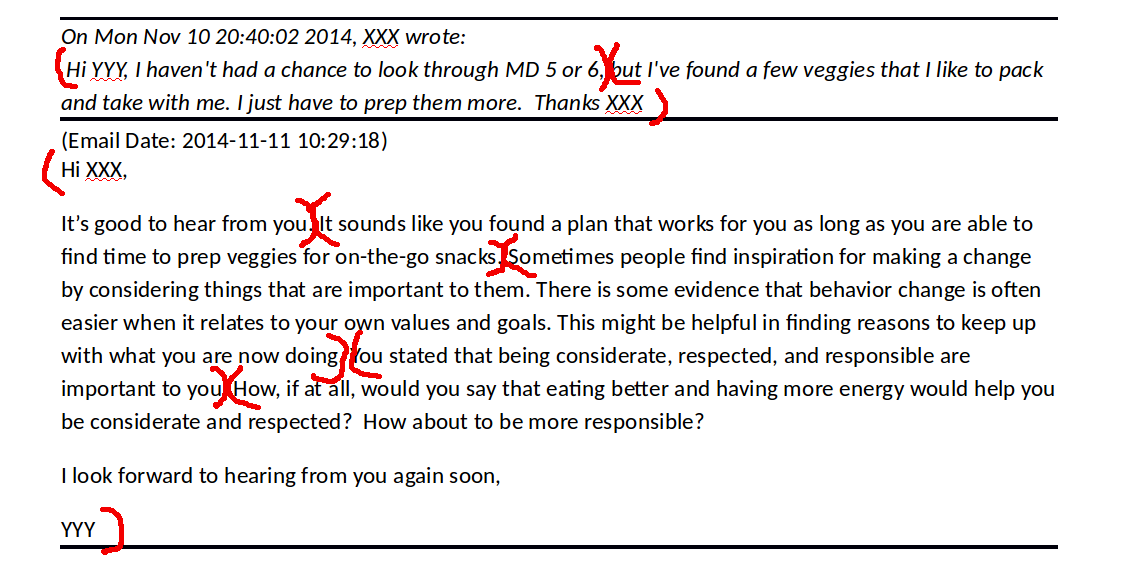
\includegraphics[width=0.9\textwidth]{figures/segment-example.png}
    \caption{\textbf{Segmentation of eCoaching text depicts the main challenges of boundary detection}.}
    \label{fig:text-segment}
\end{figure}

In this paper, we address this problem by developing several state-of-the-art machine learning based models for the segmentation of eCoaching text to promote the automatic identification of best communication strategies without human interference. More specifically, we develop Support Vector Machine (SVM), Naive Bayes (NB), K-Nearest Neighbor (KNN), Long Short Term Memory (LSTM), and Gated Recurrent Unit (GRU) by utilizing contextual, topic and punctuation mark features, to find the best model for the segmentation of eCoaching text. 

Previous studies mainly focus on segmentation of text into sections and headers\cite{apostolova2009automatic,denny2009evaluation,tepper2012statistical,cho2002text} or sentence boundary detection\cite{griffis2016quantitative,kreuzthaler2015detection,treviso2016sentence} in the medical domain. Apostolova et al.\cite{apostolova2009automatic} applied SVM by utilizing word-vector cosine similarity metric combined with several heuristics to classify clinical report into semantic sections such as demographics, history, exam procedure, finding, impression, etc. After identification of each line in the document, Tepper et al. \cite{tepper2012statistical} trained Maximum Entropy models for the section classification. In 2009, Denny et al.\cite{denny2009evaluation} proposed a SecTag algorithm, which combined natural language processing technique, terminology-based rule, and naive Bayesian score for identifying sections and headers that achieved 99\% recall with 95.6\% precision. On the other hand, SVM exploiting with linear kernel and recurrent convolutional neural networks with posodic, part of speech features and word embeddings, were trained by Kreuzthaler et al.\cite{kreuzthaler2015detection} and Griffis et al.\cite{griffis2016quantitative}, respectively, for the detection of sentence boundary. However, segmentation of clinical text, in particular, segmentation of MI or eCoaching text into groups of MI behaviors, is ignored while relying on manual hand-coded approach. Therefore, this study introduces a novel approach and the authors are not aware of any other work this approach has been considered for the segmentation of eCoaching text.  

\section*{Methods}
\subsection*{\textit{Data collection}}
The experimental dataset for this work was constructed from the 49 eCoaching sessions, which include a total of 3,138 segmented and annotated MI behaviors. Each session contains an MI intervention involving patient-provider communications in email. To filter out noise from the dataset, non-ascii characters are removed and then applied stemming to obtain a general form of word from different word representations, such as ``eating'', ``eats'', and ``eat''. We formulate the text segmentation task into a binary classification, as shown in Figure~\ref{fig:classifier}. An intervention session with email exchange is given as the input, it is partitioned into adjacent word pairs by sliding them. Each pair of them classified into either of the two categories: ``boundary'' and ``not boundary''. The text is segmented at the position, where an adjacent word pair classified into ``boundary'' class. If all pairs of word classified into ``not boundary'', the text is treated as one about a single MI behavior. Totaly, we obtained 95,421 word pairs, which include 3,138 ``boundary'' and 92,283 ``not boundary'' instances.    

\begin{figure}[!htb]
    \centering
    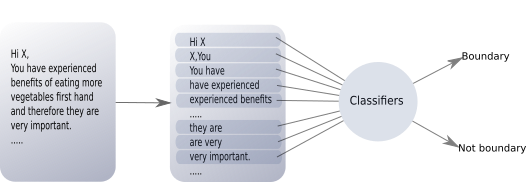
\includegraphics[width=0.80\textwidth]{figures/classifier.png}
    \caption{\textbf{Transformation of text segmentation task into text classification task}.}
    \label{fig:classifier}
\end{figure}


For the experiment, we utilized three type of features including word (textual feature), topic, and punctuation mark. Each word represented in a binary format, where 1 indicates the appearance of the word and 0 for absence. Topics are considered as features since topic models are very effective\cite{kotov2015interpretable,hashimoto2016topic,lu2016modeling} to represent text documents. In this paper, we exploit the Labeled LDA model\cite{kotov2015interpretable} and represent each word in a vector of 2 topics, where the number of topics is experimentally determined by the model performance. Punctuation mark containing one of the symbols \{`.', `,', `!', `?', `:', `;', `-'\} is also employed as feature. This is one of the most important features as they indicate the boundary of a sentence, clause, and phrase.   

\subsection*{\textit{Segmentation classifiers}}
Several state-of-the-art classifiers, including Naive Bayes (NB)\cite{pedregosa2011scikit}, Support Vector Machine (SVM)\cite{chang2011libsvm}, K-Nearest Neighbour (KNN)\cite{pedregosa2011scikit}, two variant of Recurrent Neural Networks (RNN)\cite{bengio1993problem}: Long Short Term Memory (LSTM)\cite{hochreiter1997long} and Gated Recurrent Unit (GRU)\cite{cho2014properties}, are employed to estimate the classification performance. 

\textbf{Naive Bayes}: this model is constructed by using the training data and estimate the prior probability of classes, and each feature has given the class. Then, the posterior probability is computed to predict the class label by applying the Bayes theorem with the assumption that features are conditionally independent. This study utilized a specialized version of Naive Bayes called Multinomial Naive Bayes, which is best suitable for discrete features such as word.

\textbf{Support Vector Machine}: we used this model as one of the state-of-the-art classification technique proven to perform well in text categorisation\cite{joachims1998text} for its ability to cope with very high dimensional input feature space. SVM finds the best hyperplane in the feature space that maximizes the separation between the closest ``boundary'' and ``not boundary'' training examples. In this experiment, the polynomial kernel is employed to train the SVM model for the segmentation of eCoaching text.   

\textbf{K-Nearest Neighbour}: By this model, each training sample represented as a point in the input feature space. For a new test sample, Euclidean distance is calculated to find the k-nearest neighbors. Finally, the test sample is classified into majority class of the k-nearest neighbors. We experimentally determined that best performance was achieved with k = 3 for the classification of word pairs. 

\textbf{Recurrent Neural Networks}: RNN is a neural network architecture designed to capture sequential patterns present in temporal sequence such as text data. When we predict the ``boundary'' point, adjacent word pair will help to understand the pattern of the sequence. Long Short Term Memory networks usually reffered as LSTMs\cite{hochreiter1997long}, are a special type of RNN capable of handling variable size input sequence, contains internal memory. GRU\cite{cho2014properties} is a variant of LSTM mathematically represented by the following formula:

\begin{equation}
z_t = \sigma(W_zx_t + U_zh_{t-1} + b_z)
\label{eq:firstgru}
\end{equation}
\begin{equation}
r_t = \sigma(W_rx_t + U_rh_{t-1} + b_r)
\label{eq:resetgru}
\end{equation}
\begin{equation}
\tilde h_t = tanh(W_hx_t + r_t \odot U_hh_{t-1} + b_h) 
\label{eq:candidategru}
\end{equation}
\begin{equation}
h_t = z_t \odot h_{t-1} + (1-z_t) \odot \tilde h_t
\label{eq:lastgru}
\end{equation}  
In Eq.~\ref{eq:firstgru}-\ref{eq:lastgru}, $\sigma$ corresponds to sigmoid function and $\odot$ designates an element-wise product. The update gate $z_t$ and reset gate $r_t$ at time step $t$ are computed by the Eq.~(\ref{eq:firstgru}) and~(\ref{eq:resetgru}), where $W_z$, $W_r$, $W_h$, $U_z$, $U_r$, $U_h$ are the weight matrices and $b_z$, $b_h$ and $b_r$ are bias vectors. The activation $h_t$ of the GRU at time $t$ is a linear combination of previous activation $h_{t-1}$ and the candidate activation $\tilde h_t$, which is represented by Eq.~(\ref{eq:lastgru}) and~(\ref{eq:candidategru}). We build our RNN model with one hidden layer, output layer, and input layer which get one hot encoding of word vector as input. Since one-hot vector is given in the input layer, results are reported with textual features and punctuation marks only. We experimentally determined that the best performance is achieved when the number of hidden units = 32, batch size = 8, optimizer = adam, as well as 600 epochs is used based on the validation loss.         
  
\subsection*{\textit{Evaluation metrics}}
In this experiment, standard metrics: precision, recall, and F1-measure, are applied to evaluate the performance of binary classifiers\cite{aas1999text}. However, we didn't report accuracy as a performance metric because accuracy is highly sensitive to the prior class probabilities and does not fully describe the actual difficulty of the decision problem for an unbalanced dataset. We conduct the experiment with 5 folds cross-validation and weighted macro-averaging of these metrics over the folds. All models have trained on 80\% of the word pairs and remaining 20\% of the data is used as a test set for reporting the performance of the model. We also estimated the area under the receiving operating characteristics (ROC) curve\cite{kumar2011receiver} (AUC) metric due to its effectiveness in measuring the quality of binary classifiers for imbalanced datasets\cite{hu2015kernelized}. 

\section*{Results}
Experimental results are evaluated with ``boundary'' and ``not boundary'' classes as well as their weighted average, which are shown in Table~\ref{tab:result_boundary}, \ref{tab:result_not_boundary} and \ref{tab:result_weighted_avg}, respectively.\\

\begin{table}[ht]
\centering
\caption{Performance of NB, SVM, KNN, and RNN for detecting boundaries of segmentation in eCoaching text. The highest value for each performance metric is highlighted in bold.}
\label{tab:result_boundary}
  \begin{tabular}{|l|l|l|l|p{0.15\linewidth}|p{0.15\linewidth}|l|}
  \hline
   \multirow{2}{*}{\textbf{Method}} & \multicolumn{3}{|c|}{\textbf{contextual features only}} & \multicolumn{3}{|c|}{\textbf{contextual + punctuation marks (+ topics except RNN)}} \\\cline{2-7}
   & \textbf{Precision}  & \textbf{Recall} & \textbf{F1-measure} & \textbf{Precision}  & \textbf{Recall} & \textbf{F1-measure}\\ \hline    
    
 NB & 0.594 & 0.662 & 0.626 & 0.590 & 0.666 & 0.626 \\ \hline
 SVM & 0.742 & \textbf{0.679} & 0.709 & 0.774 & 0.696 & 0.733\\ \hline
 KNN & \textbf{0.808} & 0.663 & \textbf{0.728} & \textbf{0.820} & \textbf{0.742} & \textbf{0.779}\\ \hline
 LSTM & -- & -- & -- & 0.619 & 0.416 & 0.497  \\ \hline
 GRU & -- & -- & -- & 0.642 & 0.490 & 0.554 \\ \hline 
  \end{tabular}
\end{table}                 

As follows from Table~\ref{tab:result_boundary}, KNN performs best among all machine learning models in terms of precision and F1-measure, achieved 0.808 precision with 0.728 F1-measure when contextual features are used, and 0.820 precision with 0.779 F1-measure when a combination of contextual topic, and punctuation mark features are used. However, RNN demonstrates the lowest performance among all models in terms of recall and F1-measure while GRU shows 3.72\%, 17.79\% and 11.47\% higher precision, recall, and F1-measure than LSTM. In this study, SVM appears as the second highest model in terms of precision and F1-measure, obtains highest 0.679 recall when only textual features are used. On the other hand, NB exhibits lowest precision value 0.594 but performs better than RNN with recall and F1-measure. When textual features are used in combination with topic and punctuation mark, recall increases by 0.6\%, 2.5\%, and 11.92\%, and F1-measure increases by 0\%, 3.39\%, and 7\% for NB, SVM, and KNN models, respectively. Nevertheless, precision increases by 4.31\% and 1.49\% for SVM and KNN methods while decreases by 0.7\% in NB. \\

\begin{table}[ht]
\centering
\caption{Performance of NB, SVM, KNN, and RNN  for detecting no boundaries in eCoaching text. The highest value for each performance metric is highlighted in bold.}
\label{tab:result_not_boundary}
  \begin{tabular}{|l|l|l|l|p{0.15\linewidth}|p{0.15\linewidth}|l|}
  \hline
   \multirow{2}{*}{\textbf{Method}} & \multicolumn{3}{|c|}{\textbf{contextual features only}} & \multicolumn{3}{|c|}{\textbf{contextual + punctuation marks (+ topics except RNN)}} \\\cline{2-7}
   & \textbf{Precision}  & \textbf{Recall} & \textbf{F1-measure} & \textbf{Precision}  & \textbf{Recall} & \textbf{F1-measure}\\ \hline    
    
 NB & 0.988 & 0.985 & 0.987 & 0.989 & 0.984 & 0.986 \\ \hline
 SVM & \textbf{0.989} & 0.992 & 0.991 & 0.990 & 0.993 & 0.991\\ \hline
 KNN & \textbf{0.989} & \textbf{0.995} & \textbf{0.992} & \textbf{0.991} & \textbf{0.994} & \textbf{0.993}\\ \hline
 LSTM & -- & -- & -- & 0.981 & 0.991 & 0.986 \\ \hline
 GRU & -- & -- & -- & 0.983 & 0.991 & 0.987 \\ \hline 
  \end{tabular}
\end{table}

Table~\ref{tab:result_not_boundary} summarizes the performance of NB, SVM, KNN, and RNN models for detecting ``not boundary'' class in eCoaching text. Performance is remarkably high in ``not boundary'' class compared to boundary detection. Similar to boundary detection, KNN consistently outperforms over all other methods but obtains 22.40\%, 50.07\%, and 36.26\% higher precision, recall, and F1-measure for contextual feature and 20.85\%, 33.96\%, and 27.47\% higher precision, recall, and F1-measure for combined features. However, RNN demonstrates the lowest performance and exhibits 0.981 and 0.983 precision with 0.986 and 0.987 F1-measure for LSTM and GRU, respectively. Impact of additional features is also consistent in ``not boundary'' classification. Results show that F1-measure increases by 0\%, and 0.1\% for SVM and KNN models although decreases by 0.1\% for NB. \\

\begin{table}[ht]
\centering
\caption{Weighted average performance of NB, SVM, KNN, and RNN for the segmentation of eCoaching text in detecting both ``boundary'' and ``not boundary'' classes. The highest value for each performance metric is highlighted in bold.}
\label{tab:result_weighted_avg}
  \begin{tabular}{|l|l|l|l|p{0.15\linewidth}|p{0.15\linewidth}|l|}
  \hline
   \multirow{2}{*}{\textbf{Method}} & \multicolumn{3}{|c|}{\textbf{contextual features only}} & \multicolumn{3}{|c|}{\textbf{contextual + punctuation marks (+ topics except RNN)}} \\\cline{2-7}
   & \textbf{Precision}  & \textbf{Recall} & \textbf{F1-measure} & \textbf{Precision}  & \textbf{Recall} & \textbf{F1-measure}\\ \hline    
    
 NB & 0.975 & 0.974 & 0.975 & 0.976 & 0.974 & 0.975 \\ \hline
 SVM & 0.981 & 0.982 & 0.981 & 0.983 & 0.983 & 0.983\\ \hline
 KNN & \textbf{0.983} & \textbf{0.984} & \textbf{0.983} & \textbf{0.986} & \textbf{0.986} & \textbf{0.986}\\ \hline
 LSTM & -- & -- & -- & 0.969 & 0.972 & 0.970 \\ \hline
 GRU & -- & -- & -- & 0.972 & 0.974 & 0.973 \\ \hline 
  \end{tabular}
\end{table} 

Table~\ref{tab:result_weighted_avg} outlines the weighted average results of the experiment on the models for the segmentation of eCoaching text by classifying them into ``boundary'' and ``not boundary'' classes. Overall, KNN obtains the best performance with all metrics and RNN denotes the lowest performance among all methods. NB and SVM demonstrate moderate performace, obtain precision 0.975 and 0.981, recall 0.974 and 0.982, and F1-measure 0.975 and 0.983 when textual features are used. Effect of the additional features is also consistent as above, precision increases by 0.1\%, 0.2\%, and 0.3\%, recall increases by 0\%, 0.1\%, and 0.2\%, and F1-measure increases by 0\%, 0.2\%, and 0.3\%, for NB, SVM, and KNN methods, respectively, when combined features are used.\\

\section*{Discussion}
This study is the first large-scale efforts to evaluate the segmentation of eCoaching text. Experimental results indicate that KNN is the best model among all machine learning methods considered for this study. KNN achieved 0.986 F1-measure in overall, 0.779 and 0.993 F1-measures for detecting ``boundary'' and ``not boundary'', respectively. The robust performance of KNN provides the evidence that machine learning models are capable to learn information from the email exchange. Although the domain of this study was intentionally quite small, we believe that our study is not limited to the ecoacing domain, and it can be successfully applied to other domain as well.

The additional topic and punctuation mark feature made a significant improvement in performance of all machine learning methods. In every case, the model performs better when a contextual feature is used in combination with topic and punctuation mark features. This results also mean that segmentation performance might be improved by adding more relevant features including human insight into the problem.       

\begin{figure}[!htb]
    \centering
    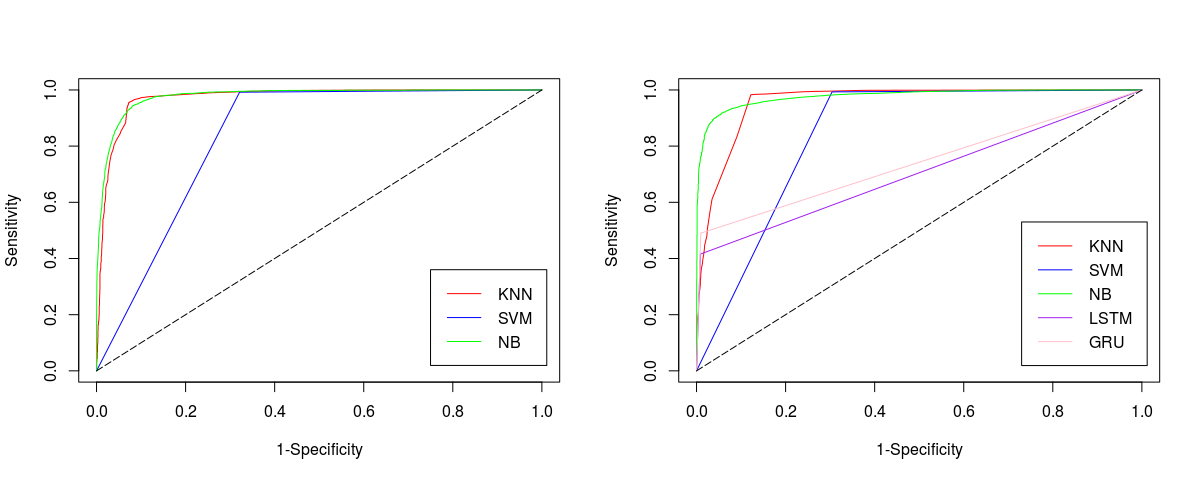
\includegraphics[width=1.0\textwidth]{figures/roc-curves.png}
    \caption{\textbf{Receiver operating characteristic curves showing the performance of binary classifiers for the segmentation of eCoaching text when textual features (left) and combination of textual and other features (right) are used}.}
    \label{fig:roc-curves}
\end{figure}

In this paper, results are reported by each class to avoid confusion about the overall model performance. In addition, standard metrics: precision, recall, and F1-measure were used to eliminate doubt about the model performance because accuracy is misleading for imbalance dataset. AUC values are also outlined due to its effectiveness in measuring the quality of binary classifiers for imbalanced datasets\cite{hu2015kernelized}, which was demonstrated by the ROC curves in Figure~\ref{fig:roc-curves}. NB shows the highest AUC values and achieved 0.978 for both cases while it provides lowest classification results except RNN. On the other hand, KNN and SVM exhibit 0.972 and 0.835 AUCs when only textual features are used; and 0.959 and 0.844 AUCs when a combination of textual, topic and punctuation mark features are used. Finally, RNN demonstrates lowest AUC values among all machine learning models, achieved AUC values 0.704 and 0.740 for LSTM and GRU, respectively. 

We observed worst results of RNN, in particular, LSTM and GRU for the text segmentation. We believe that RNN performed poorly because it has a large set of weights which required a large set of data for both classes. It this study, we utilized 3,138 examples of boundary case which failed to achieve good results. While the performance of RNN is poor, GRU performed better than LSTM which was already observed in other previous study\cite{chung2014empirical}.

Punctuation mark plays an important role in segmentation boundary detection, and large numbers of errors were encountered by the false positive of boundary identification. Similarly, additional information is the common reason for the classified original segment into multiple segments. For example, [need help from April].

Our proposed approach is novel for text segmentation of eCoaching text because previous studies focus on the segmentation of text into sections, headers, and sentences. However, this study segmented email exchange into groups of MI behavior. This work will significantly reduce the amount of resource and time required to segment email text manually. Furthermore, this paper can help to annotate each segment automatically by building a new classifier, which will accelerate the pace of finding best communication strategies to develop an effective MI intervention for healthy eating.

As for future work, As our future work, we plan to evaluate our approach on other datasets involves in discourse analysis. We also plan to use a combination of machine learning and natural language approaches to improve model performance. For example, part-of-speech tagging and distance from the boundary of the sentence might significantly enhance the classification performance. The limitation of this study is that eCoaching text is collected from a single medical institute; formatting, style, and email segment can be different in other settings.
 
\section*{Conclusion}
Segmentation of eCoaching text is an integral part of developing an automated eCoaching intervention. Although several studies have done for the segmentation of clinical text into sections and sentences, none of them are used for the segmentation of text into a groups of MI behaviors in the setting of discourse analysis with email under the principle of motivational interviews. In this paper, we compared the performance of machine learning models for the task of segmentation of e-coaching text. We found out that k-nearest neighbor provides the best performance for the segmentation of text in terms of all performance metrics. Manual segmentation of e-coaching data is very resource-intensive and time-consuming task, which can significantly decrease the time and effort required to develop effective behavioral interventions. Our proposed methods can help to identify individual text segments, which can be annotated directly with a classification model. This approach will help for developing fully automated eCoaching and also accelerate the pace of identifying effective communication strategies linked to healthy eating.


\section*{Acknowledgments}
This study was supported by a grant from the National Institutes of Health, NIDDK R21DK108071, Carcone and Kotov, MPIs. We would like to thank the student assistants in the Department of Family Medicine and Public Health Sciences at Wayne State University School of Medicine for their help in developing the training dataset by manually segmented the eCoaching text. 

\bibliographystyle{vancouver}
\bibliography{references}

\end{document}
